\chapter{Analyse}
\label{sec:analyse}
Dieses Kapitel der Arbeit betrachtet zunächst den gegenwärtigen Stand der Technik hinsichtlich bereits vorhandenen Tools. Ihre Stärken und Schwächen werden ebenfalls aufgezeigt. Danach geht es um die Anforderungsanalyse der Webanwendung. Dazu wird eine allgemeine Struktur festgelegt, wie die Arbeit systematisch aufgebaut sein soll. Anschließend wird der aktuelle Zustand (Ist-Analyse) des Projektes ermittelt und anhand dieser Ist-Analyse erfolgen die funktionalen und nicht-funktionalen Anforderungen an die zu entwickelnde Webanwendung.

\section{Stand der Technik}
\label{sec:stand der technik}
Bei der Suche nach öffentlich zugänglichen Tools für die Durchführung von Workshops wurden folgenden Ergebnisse gefunden:

\subsection{IdeaBoardz}
\label{sec:ideaBoardz}
IdeaBoardz\footnote{vgl. \url{https://ideaboardz.com/}} ist eine freie webbasierte Anwendung zum Brainstorming, Erstellen einer ToDo-Liste oder zur Retrospektive im agilen Projektmanagement. Mit diesem Tool ist eine Zusammenarbeit möglich. Die beteiligten Personen können entweder zeitgleich oder zu verschiedenen Zeiten ortsunabhängig auf das gemeinsame Dokument zugreifen und bearbeiten. In Echtzeit zusammenarbeiten, ist bei IdeaBoardz nicht realisierbar. Das hat zur Folge, dass bei der Veränderung des Zustands keine sofortige Aktualisierung der Benutzeroberfläche erfolgt. IdeaBoardz wird unter anderem bei Brainstorming-Methode wie die 6-Hüte-Methode\footnote{engl. Six Thinking Hats} von De Bono und auch für die Ideenbewertung bekannte SWOT\footnote{steht für Strengths-Weaknesses-Opportunities-Threats-Analyse}-Analyse angewendet. Die Registrierung ist optional, so dass der Nutzer auch IdeaBoardz verwenden kann, ohne sich anzumelden.

\begin{figure}[H]
  \begin{center}
    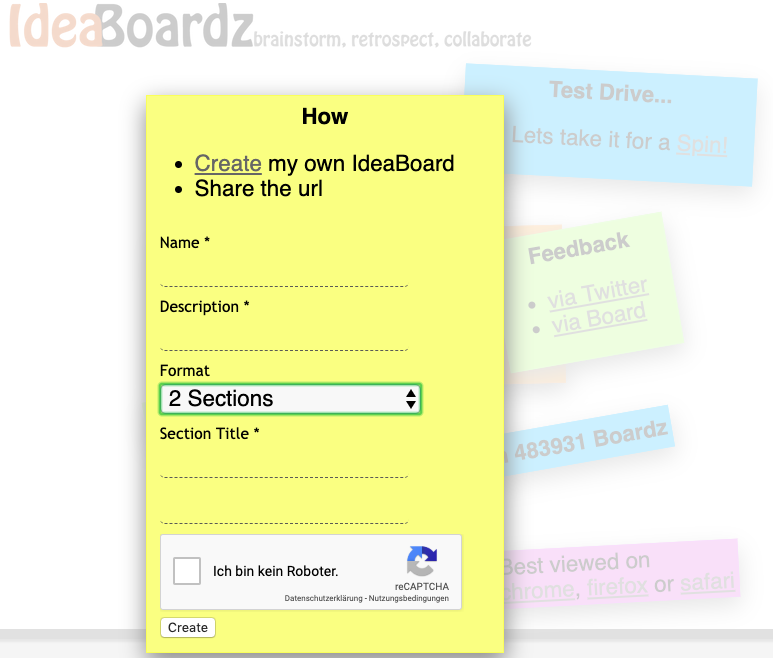
\includegraphics[scale=0.3]{img/ideaBoardz1}
	\caption{Erstellen eines eigenen IdeaBoards.} 
	\label{fig:erstellen des eigenen ideaboards}
  \end{center}   
\end{figure}

Die \textbf{Abbildung \ref{fig:erstellen des eigenen ideaboards}} zeigt, wie ein IdeaBoard zu erstellen ist. Neben dem Namen des Boards werden das Thema (Description) und Formate (Format) benötigt. Es können bis zu 10 Sektionen gewählt werden und es stehen noch weitere Formate zur Verfügung, wie Pro und Contra, ToDo-Liste, Six Thinking Hats und vieles mehr. Anschließend wird ein Titel für jegliche Sektionen eingegeben.

\begin{figure}[H]
  \begin{center}
    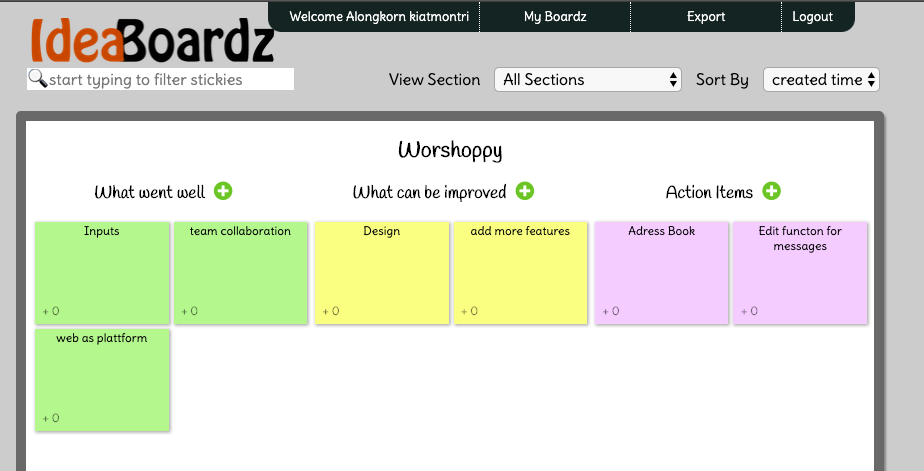
\includegraphics[scale=0.35]{img/ideaBoardz2}
	\caption{Darstellung von Sektionen} 
	\label{fig:darstellung von sektionen}
  \end{center}   
\end{figure}

Wie in \textbf{Abbildung \ref{fig:darstellung von sektionen}} zu sehen ist, sind die Eingaben in Sektionen strukturiert und farbig sortiert. Das Thema steht in der Mitte. Jede Sektion hat einen Titel und einen Plus-Button. Mit diesem Button können zu jeder Sektion neue Eingaben hinzugefügt werden. Die Eingaben werden als Karteikarten bzw. Notizzetteln visualisiert. Der weiße Hintergrund kann wie ein Whiteboard oder eine Pinnwand gesehen werden. Die Eingaben können auch von beteiligten Personen abgestimmt werden. Es ist auch möglich, die Daten nach Datum oder Abstimmung sortieren zu lassen.\bigskip

Als weiteres Feature lassen sich die Sektionen einzeln darstellen (\textbf{Abbildung \ref{fig:darstellung einer der sektionen}}). Die Suche nach dem Eingabeinhalt und das Exportieren der Ergebnisse sowohl als PDF-Datei als auch in ein Excel-Dokument werden ebenfalls bei dieser Webanwendung angeboten. Die Daten können sowohl innerhalb als auch außerhalb der Sektion zusammengeführt (Merge) werden. Ebenso lassen sich die Daten aus einer Sektion anderer Daten per Drag \& Drop zuordnen, wie in \textbf{Abbildung \ref{fig:zusammenführen und zuordnen von daten}} zu sehen ist. Mit dem Teilen von URL kann das jeweilige IdeaBoardz für die Zusammenarbeit freigegeben werden.

\begin{figure}[H]
  \begin{center}
    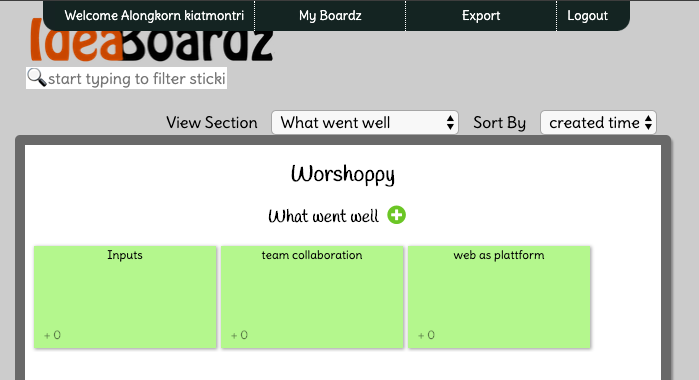
\includegraphics[scale=0.4]{img/ideaBoardz3}
	\caption{Darstellung einer der Sektionen} 
	\label{fig:darstellung einer der sektionen}
  \end{center}   
\end{figure}

\begin{figure}[H]
  \begin{center}
    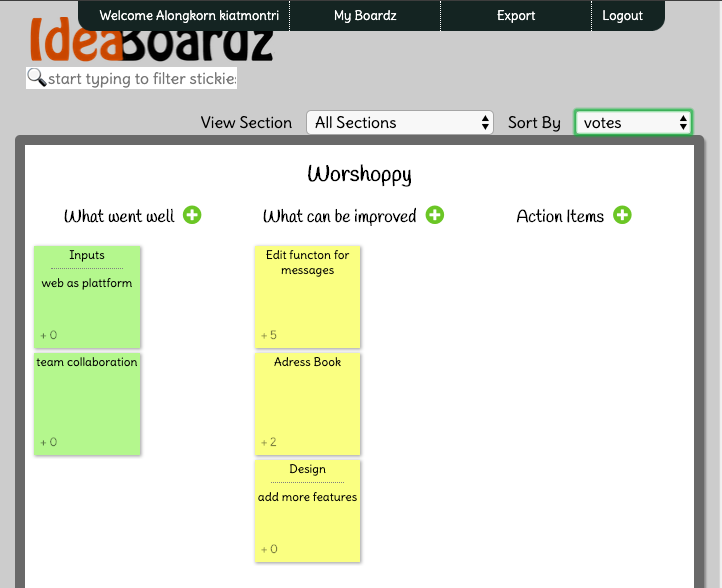
\includegraphics[scale=0.35]{img/ideaBoardz4}
	\caption{Zusammenführen und Zuordnen von Daten} 
	\label{fig:zusammenführen und zuordnen von daten}
  \end{center}   
\end{figure}

\newpage
Einige der oben dargestellten Features können für das Workshoppy-Projekt übernommen werden. Zu nennen sind:

\begin{itemize}
\item Die Eingabe wie ein Notizzettel oder Karteikarten visualisieren.
\item Die Ergebnisse als PDF-Datei exportieren.
\item Eingaben in Sektion darstellen.
\item Zuordnung von Daten (per Drag \& Drop).
\end{itemize}

Mit welchen Webtechnologien IdeaBoardz entwickelt wurde, lässt sich anhand der Informationen auf der Webseite nicht erkennen. Man kann aber davon ausgehen, dass es sich bei IdeaBoardz um eine webbasierte Anwendung mit reichlich Interaktionen auf der Benutzeroberfläche handelt, d.h. es ist über einen Webbrowser nutzbar und der Nutzer muss nichts installieren. Dementsprechend gehört IdeaBoardz zu einer Thin Client-Anwendung und zählt auch zu Rich Internet Applications sowie Web 2.0-Anwendung. (\textbf{siehe Kapitel \ref{sec:grundlagen}}).

\subsection{Miro-RealtimeBoard}
\label{sec:miro-realtimeBoard}
Miro\footnote{vgl. \url{https://miro.com/}} ist eine dynamische Webanwendung und handelt es sich um ein kollaborativer Online-Whiteboard in Echtzeit. Um das Online-Whiteboard nutzen zu können, wird ein Account benötigt. Dafür muss man sich bei Miro registrieren. Miro bietet die kostenlose Version an, sie ist für bis zu drei Teammitglieder und drei Boards geeignet.\bigskip

Begonnen wird mit einer leere Seite oder man verwendet eine von Miro bereitgestellten Vorlage. Zur Vorlage gehören unter anderem MindMap, Flowchart, Brainwriting und Concept Map. Einfügen neuer Dateien, Bilder und Dokumenten aus Google Drive oder vom Rechner ist auch möglich, um Informationen auszutauschen. Der Nutzer kann virtuelle Notizen erstellen. Die Notizen können sich nach Farbe unterscheiden und per Drag \& Drop über das komplette Board verschieben. Mit Hilfe von Share-Button vereinfacht Miro die Teilen-Funktion über eine URL oder einen Gmail-Account das ortsunabhängige und kollaborative Arbeiten in Echtzeit. Somit können die beteiligten Person beispielsweise während des Brainstormings auf die Ideen der anderen eingehen und kommentieren. Außerdem können die Benutzer das Whiteboard in eine Präsentation umwandeln oder als eine PDF-Datei exportieren.\bigskip

Miro ist ebenfalls gut geeignet zur Umsetzung eines klassischen Brainstormings (\textbf{Abbildung \ref{fig:miro board}}). Die Ideen werden in Form von Notizen erstellt. Zusammenfassend können die Notizen nach Farben kategorisiert werden.  

\begin{figure}[H]
  \begin{center}
    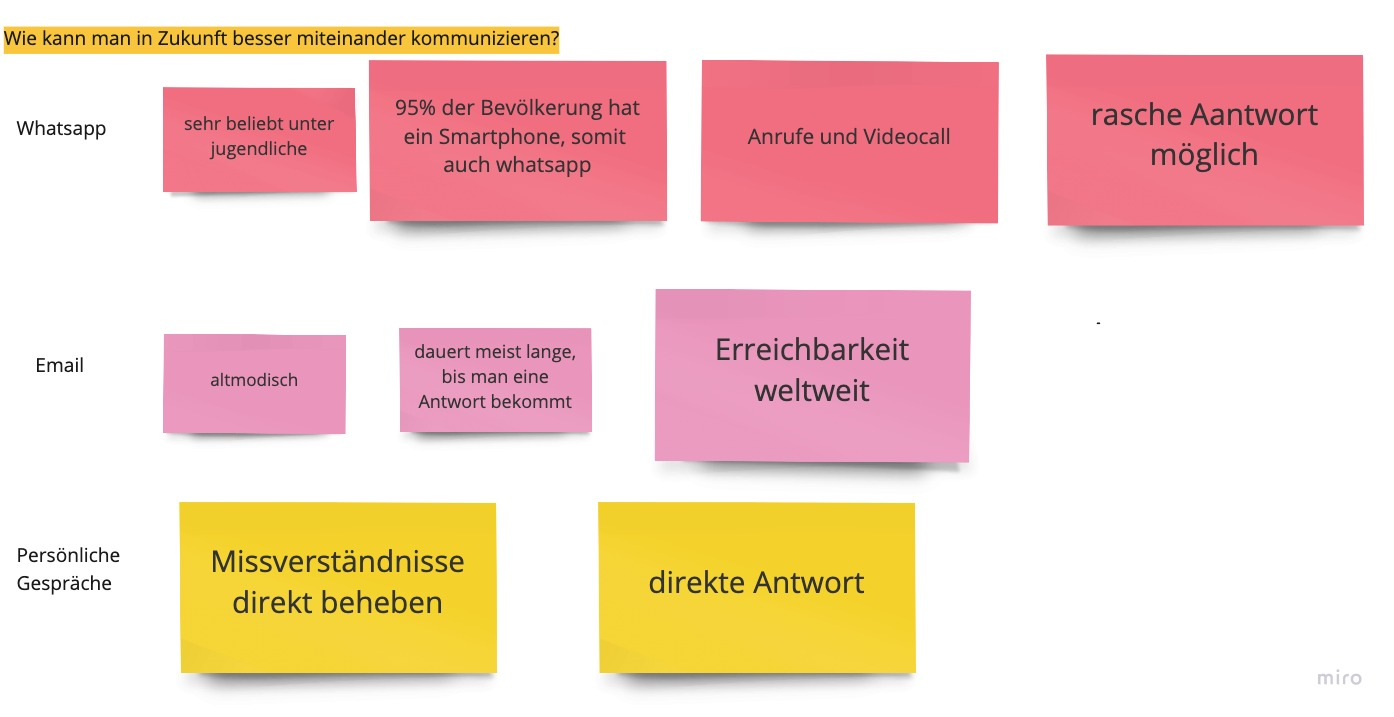
\includegraphics[scale=0.25]{img/miro1}
	\caption{Realisieren eines Brainstormings mit Hilfe von Miro} 
	\label{fig:miro board}
  \end{center}   
\end{figure}

Folgende Erkenntnisse wurden bei der Analyse von Miro gefunden und werden für das Workshoppy-Projekt übernommen: 
\begin{itemize}
\item AJAX-Anwendung
\item Thin Client-Anwendung
\item Web 2.0-Anwendung
\item Rich Internet Applications
\end{itemize}

\subsection{MindMap}
\label{sec:mindmap}
MindMap\footnote{wird häufig auch Mindmapping genannt und versteht sich als Gedankenlandkarte} zählt auch zu den Favoriten unter den Kreativitätstechniken und wird häufig in vielen Workshops als Methode zur Ideenfindung und -strukturierung eingesetzt. Man kann sie beispielsweise auch für Brainstorming, Projektplanung oder Ideensammlung verwenden.\bigskip

Bei einer Mindmap werden Begriffe und deren zugehörigen Beziehungen über eine grafische Darstellung dargestellt. Das Hauptthema oder das Schlüsselwort befindet sich als Knoten kreisförmig in der Mitte. Um das Thema herum wird alles in Form von Hauptästen notiert. Man schreibt auf jeden Hauptast ein Schlüsselwort auf. Verbunden werden sie zum Hauptthema mit Linien. Die Hauptäste bilden die ersten Gedankengänge. Von jedem Hauptast zweigen weitere Nebenäste mit Begriffen ab (\textbf{Abbildung \ref{fig:mindmap}}). 

\begin{figure}[H]
  \begin{center}
    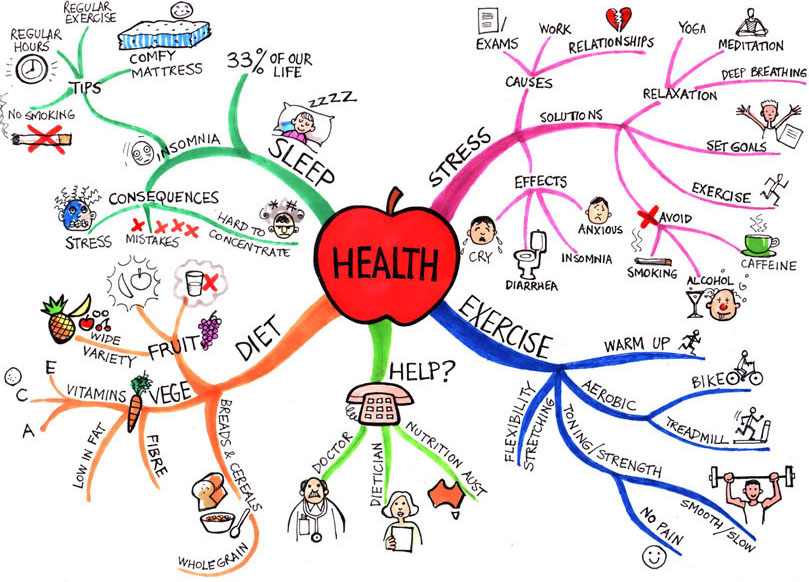
\includegraphics[scale=1.8]{img/health-mindmap}
	\caption{Health mindmap} 
	\footnotesize\sffamily\textbf{Quelle:} Learning Fundamentals: Student Study Techniques by Jane Genovese, Figure 4: Health
mindmap. Online im Internet: URL: \url{https://learningfundamentals.com.au/resources/}  
	\label{fig:mindmap}
  \end{center}   
\end{figure}

Es existieren heutzutage bereits mehrere webbasierte Mindmapping-Tools sowohl kostenlos als auch kostenpflichtig auf dem Markt. Einer von diesen ist, wie bereits im vorherigen Abschnitt vorgestellt, das \textbf{Miro-RealtimeBoard (siehe Abschnitt \ref{sec:miro-realtimeBoard})}, mit dem man Ideen visualisieren und in Echtzeit zusammenarbeiten kann. Die Übersicht zu den anderen Mindmapping-Tools kann auf dieser Webseite\footnote{\url{https://t3n.de/news/mind-mapping-online-tools-568258/}} verfolgt werden.

Neben diesen beiden dargestellten Tools, \textbf{IdeaBoardz} und \textbf{Miro}, gibt es keine weiteren nennenswerte Anwendungen. Zwar gibt es noch zahlreiche Brainstorming-Tools, die in diesem Artikel\footnote{\url{https://tallyfy.com/brainstorming-tools/}} aufgelistet sind. Jedoch sind sie meisten visuell gleich und unterscheiden sich im funktionalen Bereich wenig. Von daher geben sie keine Anreize für diese Arbeit. 

\newpage
\section{Erkennbare Stärken und Schwächen der Konkurrenz-Tools}
\label{sec:erkennbare stärken und schwächen der konkurrenzTools}
\subsection{IdeaBoardz:}
\label{sec:ideaBoardz stärken und schwächen}

\begin{itemize}
\item \textbf{Stärken:}
\begin{itemize}
\item \textbf{Zusammenfügen von Daten per Drag \& Drop:}\\
Die Daten können sowohl innerhalb als auch außerhalb einer Sektion per Drag \& Drop zusammengeführt werden.
\item \textbf{Vote-Funktion:}\\
Den Benutzern wird eine Schaltfläche geboten, mit der sie die Möglichkeit erhalten, Ihr Gefallen für Inhalte von anderen Usern oder von sich selbst auszudrücken. Vergleichbar wie Like-Button\footnote{Gefällt-mir Knopf} auf der Social Media Plattformen.
\item \textbf{Exportieren:}\\
Die Ergebnisse können sowohl als PDF- oder auch als Excel-Datei gespeichert werden.
\item \textbf{Benutzerfreundlichkeit:}\\
Die Webanwendung ist übersichtlich dargestellt, hat eine klare Strukturierung. Sie bietet außerdem eine einfache und verständliche Navigation, hat keinen unnötigen Ballast, wie z.B. Bilder, lange Texte. Sie beinhaltet außerdem kontrastreiche Farben. Die Benutzer erreichen das Ziel mit wenig Aufwand (Klick, Zeit).
\item \textbf{Keine Schulungsaufwand:}\\
Die Webanwendung ist sehr verständlich und leicht zu bedienen. Der Benutzer kommt ohne Schulung gut ans sein Ziel.
\item \textbf{Ohne Registrierung und nicht kostenpflichtig:}\\
IdeaBoardz ist eine kostenlose Webanwendung. Für die Anwendung ist keine Registrierung nötig.
\item \textbf{Responsive Webdesign:}\\
Das Layout der Website ist flexibel gestaltet, dass dieses auf dem Tablet und Smartphone eine gleichbleibende Benutzerfreundlichkeit bietet. 
Der Inhalt der Website wird auf dem mobilen Geräte einheitlich wie auf dem Laptop oder Desktop-Computer dargestellt.
\end{itemize}
\end{itemize}

\begin{itemize}
\item \textbf{Schwächen:}
\begin{itemize}
\item \textbf{Keine Möglichkeit in Echtzeit zusammenzuarbeiten:}\\
Eine der größten Nachteile von dieser Webanwendung ist, dass sie die Daten nicht in Echtzeit liefern kann.  Die Whiteboards können nicht in Echtzeit aktualisiert werden, somit verlaufen die Brainstorming-Sitzungen mit etwas Verzögerung.
\item \textbf{Keine Möglichkeit Thema oder Titel zu editieren: }\\
Das behandelte Thema und die Titel der Sektionen können nach dem Erstellen nicht mehr geändert werden.
\item \textbf{Löschen eines erstellten IdeaBoards und von Sektionen nicht möglich:}\\
Sektionen und das erstellte IdeaBoard können nicht gelöscht werden.
\item \textbf{Daten können nur einmal zusammengeführt werden:}\\
Beim ersten Zusammenführen sind die Daten fest geordnet, d.h. es ist unmöglich, sie einzeln wieder zu trennen oder mit anderen Daten zusammenzuführen. 
\end{itemize}
\end{itemize}

\subsection{Miro-RealtimeBoard:}
\label{sec:stärken und schwächen von miro}
\begin{itemize}
\item \textbf{Stärken:}
\begin{itemize}
\item \textbf{Benutzerfreundlichkeit:}\\
Die Webanwendung hat eine klare Übersicht sowie ein modernes Layout. Sie hat eine klare Strukturierung und bietet eine einfache und verständliche Navigation. Die Werkzeuge sind gut erkennbar, gut strukturiert und verständlich. Die Benutzer erreichen Ihr Ziel mit wenig Aufwand.
\item \textbf{Keine Schulungsaufwand:}\\
Die Webanwendung ist sehr verständlich und leicht zu bedienen. Der Benutzer kommt ohne große Bemühungen gut ans sein Ziel.
\item \textbf{Exportieren:}\\
Miro stellt dem Benutzer die Möglichkeit, die Ergebnisse in verschiedene Formate zu exportieren. Die Ergebnisse können sowohl als PDF- oder auch als CSV-Datei sowie als JPEG-Format gespeichert werden.
\item \textbf{Zusammenarbeit in Echtzeit:}\\
Mit Hilfe von Share-Button vereinfacht Miro die Teilen-Funktion über einen URL oder ein Gmail-Account das ortsunabhängigen und kollaborativen Arbeiten der Teammitglieder in Echtzeit.
\item \textbf{Präsentationsmodus:}\\
Die Ergebnisse können in einem Präsentationsmodus verwandeln werden.
\item \textbf{Chatfunktion:}\\
Die Teammitglieder können sich mittels einem eingebauten Chat Nachrichten untereinander austauschen.
\item \textbf{Hochladen von Dateien:}\\
Fügen neue Dateien, Bilder und Dokumente aus Google Drive oder vom Rechner ist auch möglich.
\item \textbf{Kommentar in Echtzeit hinzufügen:}\\
Durch der eingebauten Kommentarfunktion ist es möglich, das Feedback der Mitglieder in Echtzeit zu erhalten und die Qualität der Inhalte zu verbessern. 
\item \textbf{Verschiedene Vorlage:}\\
Der Benutzer hat die Möglichkeit, verschiedene Vorlagen, wie Mindmapping, User Story-Map, Flowchart, Concept-Map, Brainwriting sowie Wireframing zu verwenden.
\item \textbf{Responsive Webdesign:}\\
Das Layout der Website ist flexibel gestaltet. Das einheitliche Anzeigen von Inhalten wird auf allen Endgeräte (Laptop, Ipad, Smartphone) gewährleistet. Somit kann der Inhalt gänzlich und schnell vom Benutzer aufgenommen werden.
\end{itemize}
\end{itemize}

\begin{itemize}
\item \textbf{Schwächen:}
\begin{itemize}
\item \textbf{Registrierung notwendig:}\\
Bei dieser Webanwendung ist ein Account notwendig. Der Benutzer muss sich bei Miro registrieren.
\item \textbf{Begrenzte Funktion bei der kostenlosen Version:}\\
Die kostenlose Version ist auf bis zu drei Mitglieder und drei Boards erlaubt. Die Funktionen ist bei der kostenlosen Version begrenzt. Ein Upgrade auf 40 \$ pro Monat bringt zwei weitere Teammitglieder, unbegrenzte Boards sowie Funktionen.
\end{itemize}
\end{itemize}

Die \textbf{Tabelle \ref{tab:konkurrenten vergleich}} stellt zusammenfassend die Funktionsüberblick der beiden Konkurrenz-Tools vor.
\newcolumntype{C}[1]{>{\centering\arraybackslash}m{#1}}
\begin{table}[h]
	\centering
	\begin{tabular}{|c|c|C{3cm}|}
	\hline
	\textbf{Funktion} & \textbf{IdeaBoardz} & \textbf{Miro}\\
	\hline
	In Echtzeit zusammenarbeiten & Nein & Ja\\
	\hline
	Präsentationsmodus & Nein & Ja\\
	\hline
	Hochladen von Dateien & Nein & Ja\\
	\hline
	Vote-Funktion & Ja & Nein\\
	\hline
	Benutzerfreundlichkeit & Ja & Ja\\
	\hline
	kostenlos & volle Funktionen & begrenzte Funktionen und Mitglieder\\
	\hline
	Registrierung & Nein & Ja\\
	\hline
	Exportieren in andere Formate, z.B. in PDF-Datei & Ja & Ja\\
	\hline
	Responsive & Ja & Ja\\
	\hline
	Schulungsaufwand & Nein & Nein\\
	\hline
	Verschiedene Vorlagen, z.B. Mind Map & Nein & Ja\\
	\hline
	\end{tabular}
	 \caption{Funktionsüberblick der beiden Konkurrenzen.}
	 \label{tab:konkurrenten vergleich}
\end{table}

\section{Projektstruktur}
\label{sec:projektstruktur}
Im folgenden wird der geplante Projektablauf in Form eines Projektstrukturplans\footnote{Nach Definition der DIN 69901-5:2009 ist der Projektstrukturplan die \textit{\glqq [...] vollständige hierarchische Darstellung aller Elemente (Teilprojekte, Arbeitspakete) der Projektstruktur als Diagramm oder Liste.\grqq{}}} dargestellt:\bigskip

Auf der obersten Ebene steht das Projekt. Eine Ebene darunter die Teilprojekte oder Teilaufgaben, darunter schließlich die Arbeitspakete. Der Projektstrukturplan (\textbf{Abbildung \ref{fig:projektstruktur}}) entspricht dem typischen sequentiellen Vorgehensmodell zur Softwareentwicklung einschließlich der Entwicklung der Webanwendung. 

\begin{figure}[H]
  \begin{center}
    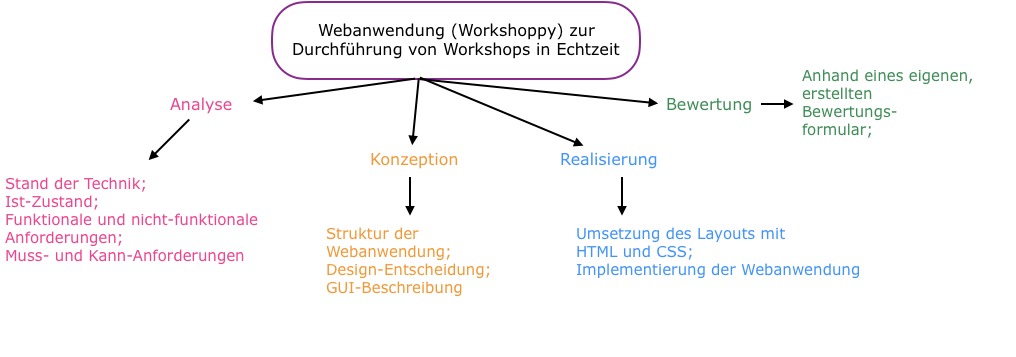
\includegraphics[scale=0.4]{img/projektstruktur}
	\caption{Projektstrukturplan} 
	\footnotesize\sffamily\textbf{Quelle:} eigene Abbildung  
	\label{fig:projektstruktur}
  \end{center}   
\end{figure}

Die Konkurrenz-Tools und eine Analyse von funktionalen, nicht-funktionalen Anforderungen sowie die Muss- und Kann-Anforderungen werden in der ersten Phase untersucht. Durch diese Analyse wird die Struktur und ein passendes Layout der Webanwendung erstellt. Die daraus entstehende Designentscheidung wird technisch in eine Webanwendung umgesetzt und am Ende wird die Webanwendung anhand eines selbst erstellten Bewertungsformulars von den Mitarbeiter im Unternehmen (mindestens 2 Personen) bewertet.

\section{Ist-Analyse}
\label{sec:istAnalyse}
Bei der Projektvorstellung wurde in der Firma zunächst über den Zustand der aktuellen Lösung für die Durchführung von Workshops gesprochen.\bigskip

Wie der Abschnitt \textbf{Stand der Technik (Abschnitt \ref{sec:stand der technik})} aufgezeigt hat, existieren bereits zahlreiche webbasierte Tools für die Durchführung von Workshops.\bigskip

Nach der Betrachtung der aktuellen Lösungen fällt das Fazit des Unternehmens folgendermaßen aus: Die beiden Tools reichen noch nicht aus, um Workshops effektiv durchzuführen. Während \textbf{IdeaBoardz} keine Zusammenarbeit in Echtzeit bieten kann, hat \textbf{Miro} bei der kostenlosen Version eine begrenzte Anzahl an Teammitgliedern, d.h. Workshops mit mehr als drei Teilnehmer muss deshalb die kostenpflichtige Version verwendet werden. Außerdem bereiten die aktuellen Lösungen viel Mühe in puncto Dateneingabe. Das bedeutet aus Sicht der Teilnehmer, dass sie erst mehrmalige \glqq Klicks\grqq{} benötigen, um Ihre Gedanken eingeben zu können.\bigskip

Als weitere und oft eingesetzte Methode zum Brainstormen in den Workshops ist das Mindmapping. Es ist eine Form, die beim Brainstorming entstehenden Ideen bildlich zu strukturieren. Jedoch hat die Mindmapping-Methode auch ihre Nachteile. Man muss sich zunächst an diese Form der Aufzeichnung gewöhnen. Denn MindMaps sehen auf den ersten Blick unübersichtlich und verschachtelt aus. Diese können sehr schnell ihre Übersichtlichkeit verlieren, wenn verschiedene Schlüsselwörter in Beziehung stehen. Demzufolge ist die Akzeptanz der Personen, die mit dieser Methode bzw. dieser Aufzeichnung nicht vertraut sind, eher gering. Es ist außerdem sehr zeitaufwendig, eine Mindmap exakt nach den Regeln zu erstellen. Mindmaps sind eher für den individuellen Gebrauch geeignet, da die verwendeten Schlüsselbegriffe und die Strukturierungen häufig für andere Personen unverständlich sind.\bigskip

Es wird von daher eine alternative Lösung benötigt, um dieses Problem zu beheben und vor allem die Durchführung von Workshops effektiver zu gestalten. Eine dieser alternativen Lösungen wäre eine benutzerfreundliche Webanwendung zu entwickeln, bei der die Teilnehmer auf ihren Endgeräten mit nur einem \glqq Klick\grqq{} ihre Gedanken eingeben können, die eine Darstellung in Echtzeit möglich machen und dem Moderator ermöglichen, die Daten digital durch eine einfach zu bedienende Benutzeroberfläche zusammenzufassen.

\section{Anforderungsanalyse}
\label{sec:anforderungsanalyse}

